
\section{Design and Implementation}

In this section we begin with a system overview of \texttt{Parikshan}. 
We then explain how it inserts test cases, into the test harness, and finally we explain how a user can use the \texttt{Parikshan} api to insert test cases in the test harness.

\begin{figure*}[t]
  \begin{center}
    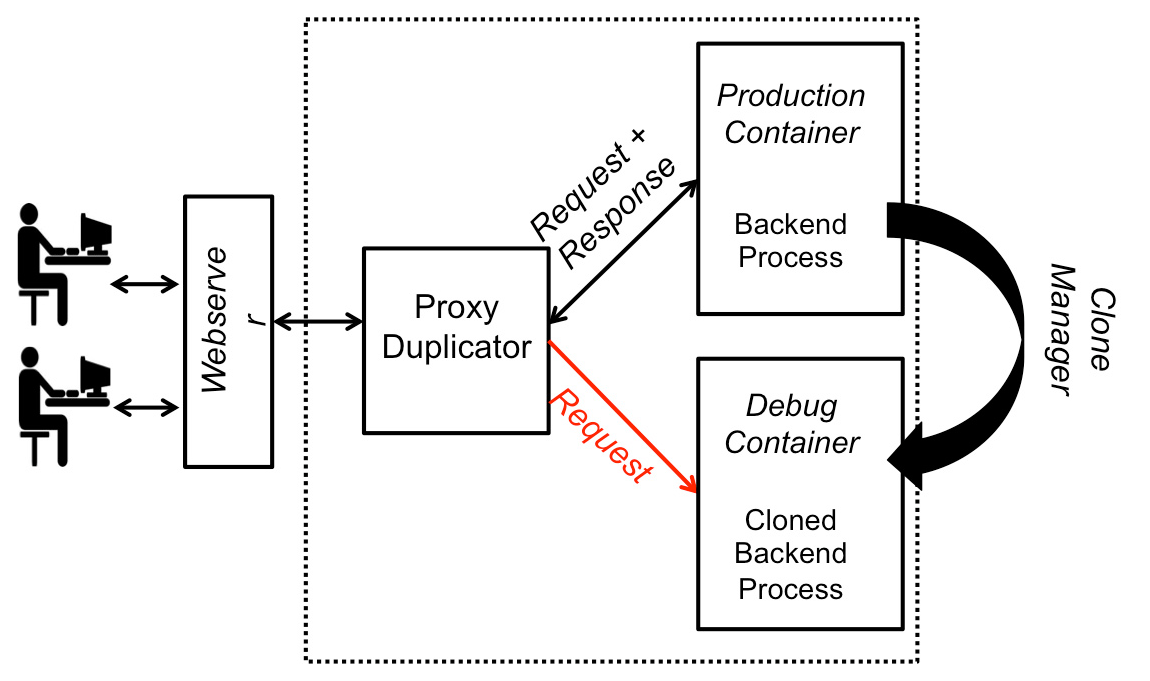
\includegraphics[width=0.8\textwidth]{figs/workflow2.eps}
    \caption{Workflow}
    \label{fig:Backend wrapped around with Parakishan Run-time}
  \end{center}
\end{figure*}


\subsection{System Overview}

There are two key components of \texttt{Parikshan} : (1) proxy network request duplicator, (2) container clone manager

